%
% $RCSfile: iterative_process.tex,v $
%
% Copyright (C) 2002-2008. Christian Heller.
%
% Permission is granted to copy, distribute and/or modify this document
% under the terms of the GNU Free Documentation License, Version 1.1 or
% any later version published by the Free Software Foundation; with no
% Invariant Sections, with no Front-Cover Texts and with no Back-Cover
% Texts. A copy of the license is included in the section entitled
% "GNU Free Documentation License".
%
% http://www.cybop.net
% - Cybernetics Oriented Programming -
%
% http://www.resmedicinae.org
% - Information in Medicine -
%
% Version: $Revision: 1.1 $ $Date: 2008-08-19 20:41:07 $ $Author: christian $
% Authors: Christian Heller <christian.heller@tuxtax.de>
%

\section{Iterative Process}
\label{iterative_process_heading}
\index{Iterative Process}
\index{Reentrant Structure}
\index{Feedback Loop}
\index{Incremental Process}
\index{Evolutionary Process}
\index{Staged Process}
\index{Spiral Process}
\index{Whirlpool Process}
\index{Rational Unified Process}
\index{RUP}
\index{Unified Modeling Language}
\index{UML}

An \emph{Iterative Process} (figure \ref{iterative_figure}) contains phases
as known from the waterfall process, supplemented by the new idea of a
\emph{Reentrant Structure} (\emph{Feedback Loop}). All phases are gone through
repeatedly, as long as the product is not satisfying. Whenever new requirements
show up, also after completion, new features can be added to the system by
reiterating a new project cycle.

\begin{figure}[ht]
    \begin{center}
        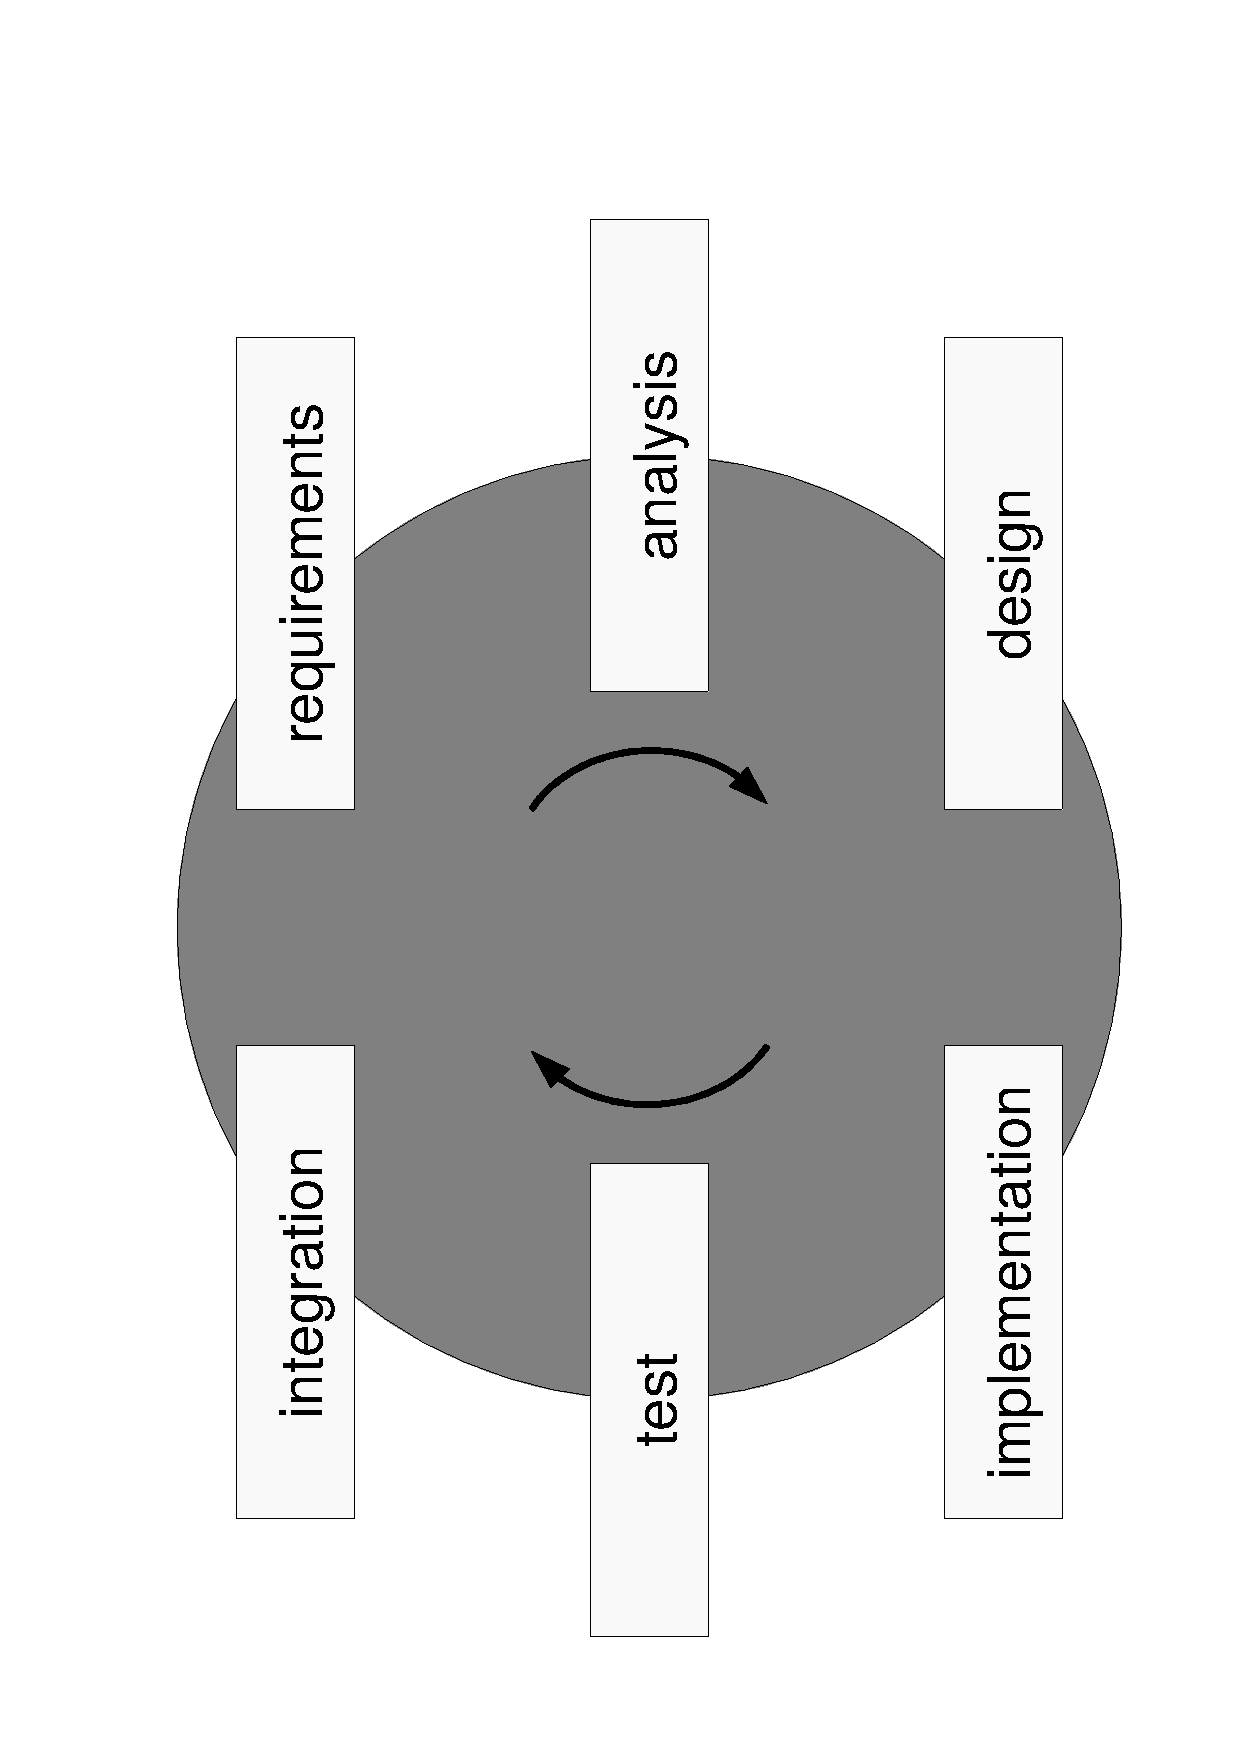
\includegraphics[scale=0.3,angle=-90]{graphic/iterative.pdf}
        \caption{Iterative Process}
        \label{iterative_figure}
    \end{center}
\end{figure}

Also here, many variations exist. They are called \emph{incremental},
\emph{evolutionary}, \emph{staged}, \emph{spiral} or \emph{whirlpool}, or
similarly. In the end, they all have their roots in some kind of
\emph{Iteration} which should \textit{frequently produce working versions of
the final system that have a subset of the required features}, as Fowler
\cite{fowlernewmethodology} writes.

A famous representative is the \emph{Rational Unified Process} (RUP) \cite{rup}.
Developed by Philippe Kruchten, Ivar Jacobson and others, RUP is the process
complement to the \emph{Unified Modeling Language} (UML). Its strength of being
a process framework that can accommodate a wide variety of processes is its
weakness, at the same time. Fowler \cite{fowlernewmethodology} criticises this
as follows:

\begin{quote}
    As a result of this process framework mentality, RUP can be used in a very
    traditional waterfall style or in an agile manner (explained in section
    \ref{agile_methodologies_heading}). So as a result you can use RUP as an
    agile process, or as a heavyweight process -- it all depends on how you
    tailor it in your environment.
\end{quote}
